%! Author = chrystal
%! Date = 06.12.19

% Preamble
\documentclass[11pt]{article}

% Packages
\usepackage{amsmath}
\usepackage{graphicx}

\chapter{Factor Analysis}

\begin{section}{Variance and Covariance}

    \subsection{Varaince-Covariance-matrix}


    \paragraph{Covariance} Hints if the result of one variable gives you information about the other $\rightarrow$
    A small standard deviation will cause a covariance near zero.
    $cov(x,y) = \frac{1}{n-1} \sum_{i=1}^n (x_i - mean_x) \times (y_i - mean_y)$ \\
    $cov(x,x) = var(x)$

    \paragraph{Variance-Covariance-matrix} square matrix that contains the variances and covariances associated with several variables x and y.
    Scatter-Plotting the Variance-Covariance-Matrix every dot represents one person, with one axes representing one variable.

    $$ S =
    \begin{bmatrix}
        $cov(x,x)$
        & $cov(x,y)$ \\
        a $cov(y,x)$
        & $cov(y,y)$
    \end{bmatrix}
    $$
    
    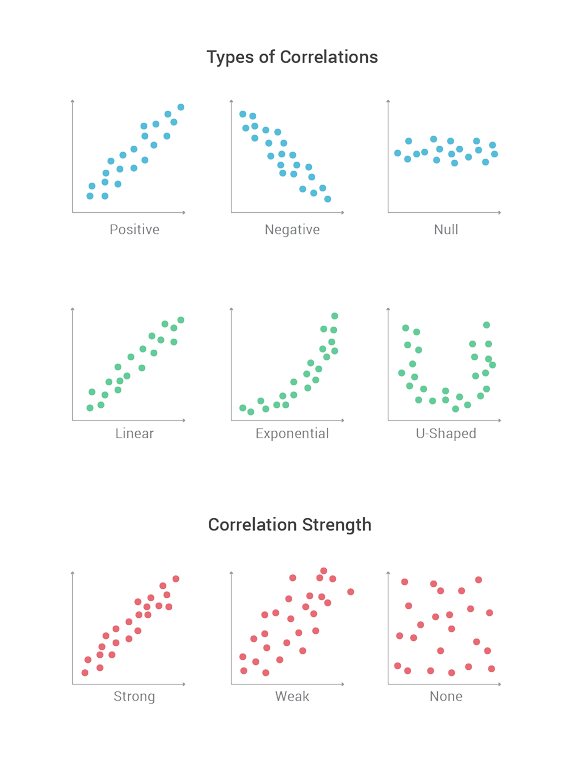
\includegraphics{../assets/scatterplots.png}

    \paragraph{Example} \textit{
    x, y: liking of course x, y. X having a high variance, Y a very low. Therefore both Covariances will be very low as well.
    A data set with low variance will not explain much $\rightarrow$ Correlation of null
    
    $$ S =
    \begin{bmatrix}
        16
        & 2.5 \\
        a 2.5
        & 2
    \end{bmatrix}
    $$
    }


    \begin{matrix}
        1 & 2 & 3\\
        a & b & c
    \end{matrix}
\end{section}